\documentclass[11pt, oneside]{article}   	% use "amsart" instead of "article" for AMSLaTeX format


% \usepackage{draftwatermark}
% \SetWatermarkText{Draft}
 % \SetWatermarkScale{5}
% \SetWatermarkLightness {0.85} 
% \SetWatermarkColor[rgb]{0.7,0,0}


\usepackage{geometry}                		% See geometry.pdf to learn the layout options. There are lots.
\geometry{letterpaper}                   		% ... or a4paper or a5paper or ... 
%\geometry{landscape}                		% Activate for for rotated page geometry
%\usepackage[parfill]{parskip}    		% Activate to begin paragraphs with an empty line rather than an indent
\usepackage{graphicx}				% Use pdf, png, jpg, or eps� with pdflatex; use eps in DVI mode
								% TeX will automatically convert eps --> pdf in pdflatex		
\usepackage{amssymb}
\usepackage{mathrsfs}
\usepackage{hyperref}
\usepackage{url}
\usepackage{authblk}
\usepackage{amsmath}
\usepackage{graphicx}
\usepackage{fixltx2e}
\usepackage{hyperref}
\usepackage{alltt}
\usepackage{color}
\usepackage{bigints}

\newcommand{\argmax}{\operatornamewithlimits{argmax}}
\newcommand{\argmin}{\operatornamewithlimits{argmin}}


\title{What is Rejection Sampling?}
\author{David Meyer \\ dmm@\{1-4-5.net,uoregon.edu,brocade.com,...\}}

% \date{September 30, 2015}							% Activate to display a given date or no date


\begin{document}
\maketitle

\section{Introduction} 
\label{sec:intro}
Suppose that we want to sample from a distribution $f(x)$ that is difficult or impossible to sample from directly. Instead of trying to sample from $f(x)$, can we use a simpler distribution $q(x)$ from which sampling is easier? Perhaps, and the idea behind Rejection Sampling (aka Acceptance-rejection sampling) is to sample from $q(x)$ and apply some rejection/acceptance criterion such that the samples that are accepted are distributed according to $f(x)$.

\subsection{Envelope distribution and rejection criterion}

In order to be able to reject samples from $q(x)$ that aren't (approximately)   sampled from $ f(x)$, $q(x)$ must “cover” or envelop the distribution $f(x)$. This is generally done by choosing a constant $c > 1$ such that  $cq(x) > f(x)$, for all $x$. For this reason $cq(x)$ is often called the \emph{envelope distribution}. A common criterion for accepting samples from $x \sim q(x)$ is based on the ratio of the target distribution to that of the envelope distribution. The samples are accepted if

\begin{flalign}
\frac{f(x)}{cq(x)} > u
\end{flalign}

\noindent
where $u \sim Unif(0,1)$, and rejected otherwise. If the ratio is close to one, then $f(x) $ must have a large amount of probability mass around $x$ and that sample should  be more likely accepted. If the ratio is small, then it means that $f(x)$ has low probability mass around $x$ and we should be less likely to accept the sample. See Figure~\ref{fig:rgr}.  I think...



\begin{figure}
\center{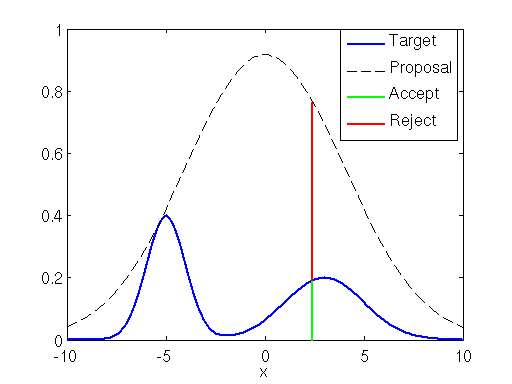
\includegraphics[scale=0.75]{images/rejectionsamplingcriterion.png}}
\caption{Rejection Sampling with a Normal proposal distribution}
\label{fig:rgr}
\end{figure}



\end{document} 

